\documentclass[fleqn]{article}
\usepackage{amsmath}
\usepackage[utf8]{inputenc}
\usepackage{graphicx}
\usepackage{enumerate}
\usepackage{fancyhdr}
\usepackage{empheq}

%plotting
\usepackage{pgfplots}
\usepackage{tikz}
\usetikzlibrary{arrows, positioning, calc}
\pgfplotsset{compat=1.12}

\setlength{\parskip}{\baselineskip}%
\setlength{\parindent}{0pt}%

\pagestyle{fancy}
\fancyhf{}
\rhead{Henrik Samuelsson, 7304294973}
\lhead{Lösning av Inlämningsuppgift}

\begin{document}

\begin{titlepage}
\title{Lösning av Inlämningsuppgift \\ Matematik 1 för produktutveckling, MA1439 \\ Lp 2, Ht 15}
\author{Henrik Samuelsson}
\maketitle
\thispagestyle{empty}
\end{titlepage}

\section*{Uppgift 1.}
Förenkla nedanstående uttryck så långt det går
\[
\dfrac{x^2 - 9}{x - 1} \cdot \dfrac{x^2 - 2x + 1}{x + 3}
\]

\textbf{Lösning}

Börja med skriva om uttrycket genom att  faktorisera de båda täljarna. Vi använder konjugatregeln och en av kvadreringsreglerna när vi faktoriserar. Resultatet blir
\[
\dfrac{(x + 3)(x-3)}{x - 1} \cdot \dfrac{(x-1)^2}{x + 3}
\]
Det går nu att eliminera båda nämnarna i uttrycket genom att stryka mot motsvarande termer i täljarna. Vi får kvar följande förenklade uttryck
\[
$(x-3)(x-1)$
\]
\textbf{Svar}

Det förenklade uttrycket blir $(x-3)(x-1)$

\newpage

\section*{Uppgift 2.}

Lös ekvationssystemet
\begin{empheq}[left = \empheqlbrace]{align}
&x + y + 2z = 9\\
&3x - y + z = 4\\
&x - 2y - 3z = -12
\end{empheq}

\textbf{Lösning}

Vi vill i ett första steg få ner ekvationssystemet till ett system med två ekvationer och två obekanta. Vi väljer att använda additionsmetoden för att få bort y ur ekvationssystemet.
 
Addera ekvation (1) med ekvation (2)
\[
x + y + 2z + 3x - y + z = 9 + 4
\]
\[
4x + 3z = 13
\]

Addera ekvation (3) med ekvation (2) multiplicerad med -2
\[
x - 2y - 3z - 6x + 2y - 2z = -12 - 2 \cdot 4 
\]
\[
-5x - 5z = -20
\]
\[
x + z = 4
\]

Vi har nu ett nytt mindre ekvationssystem
\begin{empheq}[left = \empheqlbrace]{align}
&4x + 3z = 13\\
&x + z = 4
\end{empheq} 

Addera ekvation (4) med ekvation (5) multiplicerad med -3
\[
4x + 3z -3x -3z = 13 -3 \cdot 4
\]
\[
x = 1
\]
Vi vet att x är 1 och använder detta i ekvation (5) för att få fram vad z är
\[
1 + z = 4
\]
\[
z = 3
\]
Nu vet vi att x är 1 och z är 3 och använder detta i ekvation (1) för att får fram vad y är
\[
1 + y + 2 \cdot 3 = 9
\]
\[
y = 2
\]
Vi har därmed löst hela det ursprungliga ekvationssystemet.

\textbf{Svar}

x = 1, y = 2, z = 3

\newpage

\section*{Uppgift 3.}

\begin{enumerate}[(a)]
\item En andragrads-kurva har en minimipunkt då x = 5. Kurvan skär x-axeln då x = 7 och då x = a. Vilket är talet a?
\item Finn ett uttryck för en andragrads-funktion som uppfyller kraven från första delen av uppgiften.
\end{enumerate}

\textbf{Lösning}
\begin{enumerate}[(a)]
\item
Vi har tre olika värden på x-axeln att hålla reda på i den här uppgiften. Låt oss kalla dessa värden $x_v$, $x_b$ och $x_a$.

$x_v = 5$ kurvan har här sin minimipunkt, det vill säga kurvan vänder av uppåt på båda sidor av detta värde på x-axeln.

$x_b = 7$ kurvan skär här x-axeln.

$x_a = a$ detta är den andra platsen som kurvan skär x-axeln och det värde som vi söker.

Eftersom $x_v$ är mindre än $x_b$ och så måste minimipunkten ligga under x-axeln, vi vet ju att kurvan vänder uppåt på båda sidor av minimipunkten. Vi vet därmed också att den saknade skärningspunkten med x-axeln ligger till höger om både $x_v$ och $x_b$.

Den sista pusselbit som vi behöver är det faktum att andragradskurvor är symmetriska. Det betyder att avståndet mellan $x_v$ och $x_b$ är lika stort som det kända avståndet mellan $x_v$ och $x_b$ det vill säga 2.

Vi således att $x_a = 5 - 2 = 3$.

\textbf{Svar}

Talet a är 3. 

\item
Vi vet från första delen av uppgiften att andragradsfunktionen är noll när x är 3 och när x är 7. Det vill säga funktionen kan skrivas som
\[
f(x) = (x-3)(x-7) = x^2 - 7x - 3x + 21 = x^2 - 10x + 21  
\]
Vi plottar en graf av funktionen för att kontrollera att vi har tänkt rätt.

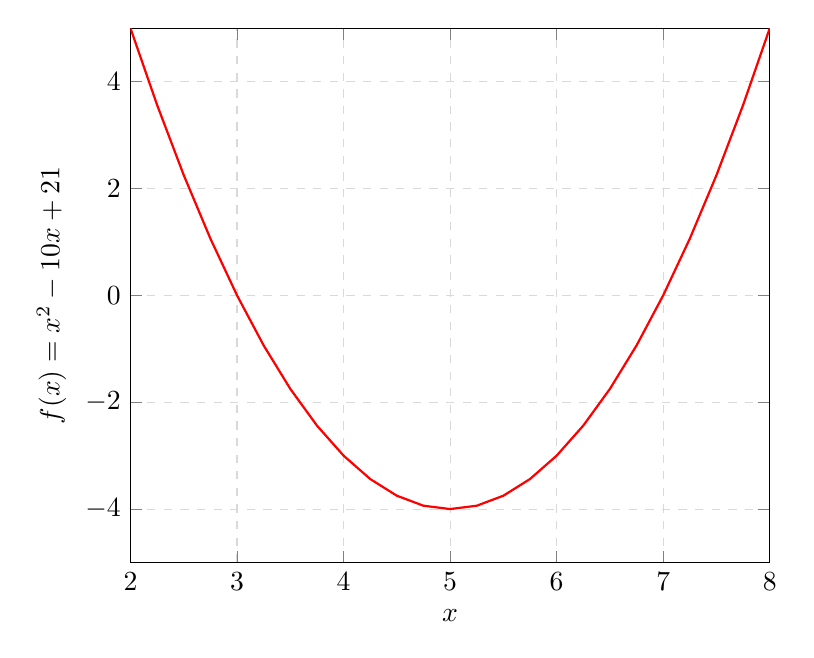
\begin{tikzpicture}
	\begin{axis}[
	 	width=0.8\textwidth,
		xlabel=$x$,
		ylabel={$f(x) = x^2 - 10x + 21 $},
		domain=2:8,
 		grid = major,
        grid style={dashed, gray!30},
		xmin=2,     % start the diagram at this x-coordinate
        xmax=8,    % end   the diagram at this x-coordinate
        ymin=-5,     % start the diagram at this y-coordinate
        ymax=5,   % end   the diagram at this y-coordinate
	]
    % use TeX as calculator:
	\addplot [mark = none, red ,thick]{x^2 - 10*x + 21}; 
	\end{axis}
\end{tikzpicture} 

Ser korrekt ut, grafen skär x-axeln vid $x=3$ och $x=7$ och minimipunkten inträffar då $x=5$.

\textbf{Svar}
\[
f(x) = x^2 - 10x + 21
\]

\newpage

\end{enumerate}

\end{document}
